\documentclass[12pt]{beamer}
\usetheme{metropolis} % Tema moderno y limpio

\usepackage[spanish]{babel}
\usepackage[utf8]{inputenc}
\usepackage[T1]{fontenc}
\usepackage{graphicx}
\usepackage{listings}
\usepackage{xcolor}
\usepackage{tikz} % Para colocar logo en todas las diapositivas
% Cargar hyperref al final para evitar conflictos
\usepackage{bookmark}

% Configuración de hyperref
\hypersetup{
    pdfencoding=auto,
    unicode=true,
    bookmarks=true,
    bookmarksopen=true,
    colorlinks=true,
    linkcolor=blue,
    filecolor=magenta,
    urlcolor=cyan,
    pdftitle={Sistema de Gestión de Restaurante},
    pdfpagemode=UseOutlines
}

% Ajustes para reducir espaciado vertical
\makeatletter
\setlength{\parskip}{0pt}
\beamer@compresstrue
\makeatother

% Ajustes para el tema metropolis
\metroset{
    block=fill,
    progressbar=foot,
    sectionpage=progressbar,
    numbering=fraction
}

% Configuración adicional para beamer
\setbeamersize{text margin left=0.5cm,text margin right=0.5cm}
\addtobeamertemplate{frametitle}{\vspace*{-0.5cm}}{}
\addtobeamertemplate{frame}{\vspace*{-0.5cm}}{}

% --- Configuración de Listings para código Python ---
\definecolor{codegreen}{RGB}{78,154,6}
\definecolor{codegray}{RGB}{136,138,133}
\definecolor{codepurple}{RGB}{92,53,102}
\definecolor{backcolour}{RGB}{40,42,46}
\definecolor{codefg}{RGB}{255,255,255}

\lstdefinestyle{mystyle}{
    backgroundcolor=\color{backcolour},
    commentstyle=\color{codegreen},
    keywordstyle=\color{codepurple},
    numberstyle=\tiny\color{codegray},
    stringstyle=\color{codegreen},
    basicstyle=\ttfamily\tiny\color{codefg},
    breakatwhitespace=false,
    breaklines=true,
    captionpos=b,
    keepspaces=true,
    showspaces=false,
    showstringspaces=false,
    showtabs=false,
    tabsize=2,
    frame=single,
    frameround=tttt,
    framesep=3pt,
    numbers=left,
    numbersep=8pt,
    xleftmargin=15pt,
    literate={á}{{\'a}}1 {é}{{\'e}}1 {í}{{\'i}}1 {ó}{{\'o}}1 {ú}{{\'u}}1
             {Á}{{\'A}}1 {É}{{\'E}}1 {Í}{{\'I}}1 {Ó}{{\'O}}1 {Ú}{{\'U}}1
             {ñ}{{\~n}}1 {Ñ}{{\~N}}1
}
\lstset{style=mystyle}

% --- Logo en la esquina inferior derecha de cada diapositiva ---
\setbeamertemplate{background}{%
    \begin{tikzpicture}[remember picture,overlay]
        \node[anchor=south east, xshift=-0.3cm, yshift=0.3cm] 
        at (current page.south east) {
\includegraphics[height=0.8cm]{images/logo_uct.png}};
    \end{tikzpicture}%
}

% --- Información del Título ---
\title{Sistema de Gestión de Restaurante}
\author{%
    \textbf{Integrantes:}\\[0.3cm]
    Joaqu\'{i}n Carrasco Dur\'{a}n\\[0.3cm]
    Benjamin Cabrera\\[0.3cm]
    Leonardo Ch\'{a}vez\\[0.3cm]
    \textbf{Profesor:} Guido Mellado\\[0.3cm]
    \textbf{Asignatura:} Programaci\'{o}n II\\[0.3cm]
    \textbf{Secci\'{o}n:} 2%
}

\begin{document}

% --- Portada ---
\begin{frame}
  \titlepage
\end{frame}

% --- Tabla de Contenidos ---
\begin{frame}{Contenido}
  \tableofcontents
\end{frame}

% --- Diagramas de Flujo ---
\section{Arquitectura del Sistema}
\begin{frame}{Flujo de Procesos - Carga de Ingredientes}
  \begin{center}
    \begin{tikzpicture}[node distance=1.5cm]
      % Nodos
      \node[draw, rounded corners, fill=blue!10] (csv) {Archivo CSV};
      \node[draw, rounded corners, fill=green!10, right of=csv, xshift=2cm] (pandas) {DataFrame};
      \node[draw, rounded corners, fill=yellow!10, below of=pandas] (validacion) {Validación};
      \node[draw, rounded corners, fill=red!10, left of=validacion, xshift=-2cm] (objetos) {Ingredientes};
      \node[draw, rounded corners, fill=purple!10, below of=validacion] (stock) {Stock};
      
      % Flechas y etiquetas
      \draw[->, thick] (csv) -- (pandas) node[midway, above] {\small pd.read\_csv};
      \draw[->, thick] (pandas) -- (validacion) node[midway, right] {\small verificar};
      \draw[->, thick] (validacion) -- (objetos) node[midway, above] {\small crear};
      \draw[->, thick] (objetos) -- (stock) node[midway, left] {\small agregar};
      
      % Ciclo de actualización
      \draw[->, thick, dashed] (stock) to [out=0, in=-45] node[right] {\small actualizar} (validacion);
    \end{tikzpicture}
  \end{center}
  
  \begin{itemize}[<+->]
    \item El sistema valida el formato del CSV
    \item Crea objetos Ingrediente para cada fila
    \item Actualiza el stock y la interfaz
    \item Maneja errores en cada paso
  \end{itemize}
\end{frame}

\begin{frame}{Flujo de Procesos - Gestión de Pedidos}
  \begin{center}
    \begin{tikzpicture}[node distance=2cm]
      % Nodos principales
      \node[draw, rounded corners, fill=blue!10] (menu) {Menú};
      \node[draw, rounded corners, fill=green!10, right of=menu, xshift=2cm] (pedido) {Pedido};
      \node[draw, rounded corners, fill=yellow!10, below of=pedido] (stock) {Stock};
      \node[draw, rounded corners, fill=red!10, right of=pedido, xshift=2cm] (facade) {BoletaFacade};
      \node[draw, rounded corners, fill=purple!10, below of=facade] (pdf) {PDF};
      
      % Flechas del flujo principal
      \draw[->, thick] (menu) -- node[above] {\small seleccionar} (pedido);
      \draw[->, thick] (pedido) -- node[right] {\small verificar} (stock);
      \draw[->, thick] (pedido) -- node[above] {\small generar} (facade);
      \draw[->, thick] (facade) -- node[right] {\small crear} (pdf);
      
      % Flujo de retorno
      \draw[->, thick, dashed] (stock) to [out=180, in=-135] node[left] {\small actualizar} (menu);
    \end{tikzpicture}
  \end{center}
  
  \begin{itemize}[<+->]
    \item Usuario selecciona productos del menú
    \item Sistema verifica disponibilidad en stock
    \item Se genera la boleta a través del Facade
    \item Se crea y muestra el PDF
  \end{itemize}
\end{frame}

\begin{frame}{Diagrama de Clases - Estructura Principal}
  \begin{center}
    \begin{tikzpicture}[node distance=2cm]
      % Definición de estilos
      \tikzstyle{clase}=[draw, rounded corners, fill=blue!10, minimum width=2.5cm, minimum height=1cm]
      \tikzstyle{interface}=[draw, rounded corners, fill=green!10, minimum width=2.5cm, minimum height=1cm]
      
      % Clases principales
      \node[clase] (restaurante) at (0,0) {Restaurante};
      \node[clase] (stock) at (-3,-2) {Stock};
      \node[clase] (pedido) at (0,-2) {Pedido};
      \node[clase] (boleta) at (3,-2) {BoletaFacade};
      
      % Interfaces y clases auxiliares
      \node[interface] (imenu) at (-3,2) {IMenu};
      \node[clase] (elemento) at (0,2) {ElementoMenu};
      \node[clase] (ingrediente) at (3,2) {Ingrediente};
      
      % Conexiones
      \draw[->] (restaurante) -- (stock);
      \draw[->] (restaurante) -- (pedido);
      \draw[->] (restaurante) -- (boleta);
      \draw[->] (elemento) -- (imenu);
      \draw[->] (elemento) -- (ingrediente);
      \draw[->] (stock) -- (ingrediente);
      \draw[->] (pedido) -- (elemento);
      
      % Etiquetas de relación
      \node[font=\small] at (-1.5,0.5) {usa};
      \node[font=\small] at (0,0.5) {contiene};
      \node[font=\small] at (1.5,0.5) {genera};
      \node[font=\small] at (-1.5,2) {implementa};
      \node[font=\small] at (1.5,2) {requiere};
    \end{tikzpicture}
  \end{center}
  
  \begin{itemize}[<+->]
    \item Arquitectura modular y desacoplada
    \item Uso de patrones de diseño (Facade, Strategy)
    \item Interfaces para abstracción
    \item Gestión centralizada de recursos
  \end{itemize}
\end{frame}

% ==========================================
\section{Introducción}
% ==========================================
\begin{frame}{Introducción y Objetivo}
  \begin{block}{Objetivo del Sistema}
    \onslide<1->{Desarrollar una aplicación de escritorio integral para la gestión de un restaurante}
    \onslide<2->{utilizando Python y una interfaz gráfica moderna.}
  \end{block}

  \pause\begin{alertblock}{Características Principales}
    \begin{itemize}[<+->]
      \item \alert{Gestión de inventario} de ingredientes
      \item \alert{Toma y seguimiento} de pedidos de clientes
      \item \alert{Generación automática} de menús y boletas en PDF
      \item Interfaz de usuario \alert{intuitiva} y fácil de utilizar
    \end{itemize}
  \end{alertblock}
\end{frame}

\begin{frame}{Requisitos Funcionales}
  \begin{columns}[t]
    \begin{column}{0.5\textwidth}
      \begin{exampleblock}{Gestión de Inventario}
        \begin{itemize}[<+->]
          \item Carga masiva de ingredientes vía CSV
          \item Agregar/eliminar ingredientes manualmente
          \item Control de stock en tiempo real
          \item Validación de disponibilidad
        \end{itemize}
      \end{exampleblock}
      
      \begin{exampleblock}{Gestión de Pedidos}
        \begin{itemize}[<+->]
          \item Selección visual de menús
          \item Actualización automática de stock
          \item Cálculo dinámico del total
          \item Múltiple selección de productos
        \end{itemize}
      \end{exampleblock}
    \end{column}
    
    \begin{column}{0.5\textwidth}
      \begin{exampleblock}{Generación de Documentos}
        \begin{itemize}[<+->]
          \item Carta de menú en PDF
          \item Boletas de venta
          \item Visualización integrada
          \item Almacenamiento histórico
        \end{itemize}
      \end{exampleblock}
      
      \begin{exampleblock}{Interfaz de Usuario}
        \begin{itemize}[<+->]
          \item Diseño moderno con CustomTkinter
          \item Sistema de pestañas intuitivo
          \item Retroalimentación visual
          \item Manejo de errores amigable
        \end{itemize}
      \end{exampleblock}
    \end{column}
  \end{columns}
\end{frame}

% ==========================================
\section{Arquitectura y Diseño}
% ==========================================
\begin{frame}{Arquitectura del Sistema}
  \begin{figure}
    \centering
    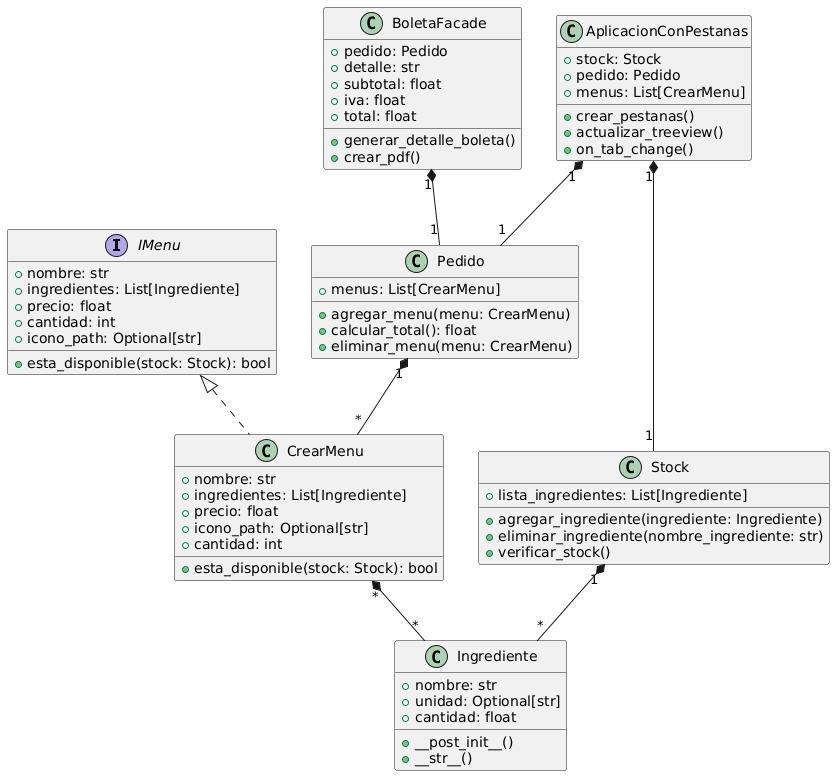
\includegraphics[width=\linewidth, height=0.8\textheight, keepaspectratio]{images/diagrama.png}
    \caption{Diagrama de clases principal del sistema.}
  \end{figure}
\end{frame}

\begin{frame}{Patrones de Diseño}
  \begin{columns}[t]
    \begin{column}{0.5\textwidth}
      \begin{exampleblock}{Facade}
        \only<1>{
          \begin{center}
            \texttt{BoletaFacade}\\[0.3em]
            \downarrow\\[0.3em]
            Simplifica la generación\\
            de boletas en PDF
          \end{center}
        }
      \end{exampleblock}
      
      \begin{exampleblock}{Factory}
        \only<2>{
          \begin{center}
            \texttt{get\_default\_menus()}\\[0.3em]
            \downarrow\\[0.3em]
            Centraliza la creación\\
            de menús predefinidos
          \end{center}
        }
      \end{exampleblock}
    \end{column}
    
    \begin{column}{0.5\textwidth}
      \begin{exampleblock}{Immutable Object}
        \only<3>{
          \begin{center}
            \texttt{CrearMenu}\\[0.3em]
            \downarrow\\[0.3em]
            Garantiza consistencia\\
            de datos
          \end{center}
        }
      \end{exampleblock}
      
      \begin{exampleblock}{Observer}
        \only<4>{
          \begin{center}
            GUI $\leftrightarrow$ Datos\\[0.3em]
            $\downarrow$\\[0.3em]
            Sincronización\\
            automática
          \end{center}
        }
      \end{exampleblock}
    \end{column}
  \end{columns}
\end{frame}

\begin{frame}{Explicación del Diagrama}
  \begin{center}
    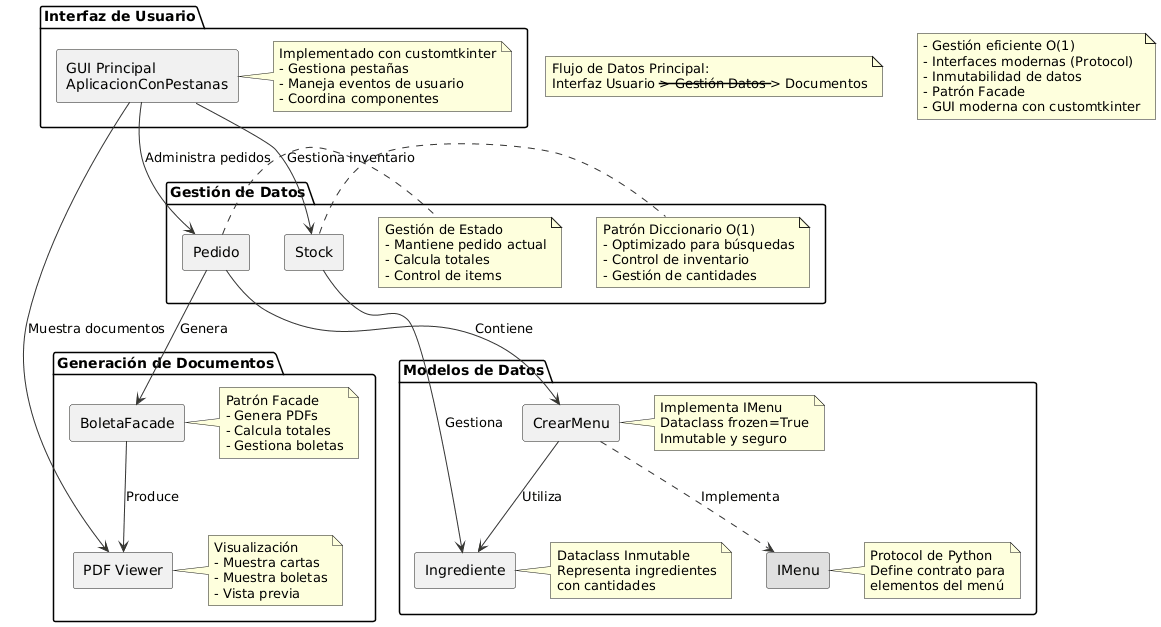
\includegraphics[width=\linewidth, height=0.8\textheight, keepaspectratio]{images/explicacion_diagrama.png}
  \end{center}
\end{frame}

% ==========================================
\section{Análisis Detallado por Pestañas}
% ==========================================

% --- Pestaña: Carga de Ingredientes ---
\begin{frame}[fragile]{Pestaña: Carga de Ingredientes}
  \begin{columns}[t]
    \begin{column}{0.4\textwidth}
      \begin{block}{Funcionalidades}
        \begin{itemize}[<+->]
          \item Carga masiva vía CSV
          \item Validación de datos
          \item Visualización previa
          \item Gestión de errores
        \end{itemize}
      \end{block}
      
      \begin{alertblock}{Flujo Interno}
        \begin{enumerate}[<+->]
          \item Selección de archivo
          \item Lectura con pandas
          \item Validación de columnas
          \item Creación de objetos
          \item Actualización de stock
        \end{enumerate}
      \end{alertblock}
    \end{column}
    
    \begin{column}{0.6\textwidth}
      \begin{exampleblock}{Código Relevante}
        \begin{lstlisting}[style=mystyle]
def cargar_csv(self):
    archivo = filedialog.askopenfilename(
        filetypes=[("CSV files", "*.csv")]
    )
    if archivo:
        try:
            self.df_csv = pd.read_csv(archivo)
            if not all(col in self.df_csv.columns 
                      for col in ['nombre', 'unidad', 'cantidad']):
                CTkMessagebox(
                    title="Error",
                    message="Formato CSV inválido"
                )
                return
            self.mostrar_dataframe_en_tabla()
        except Exception as e:
            CTkMessagebox(
                title="Error",
                message=f"Error: {str(e)}"
            )
        \end{lstlisting}
      \end{exampleblock}
    \end{column}
  \end{columns}
\end{frame}
  \begin{itemize}
    \item \textbf{Bot\'{o}n ``Cargar CSV'':} Abre un di\'{a}logo para seleccionar un archivo. En el backend, la función \texttt{cargar\_csv()} usa \textit{pandas} para leer los datos, crear objetos \texttt{Ingrediente} y agregarlos al \texttt{Stock}.
    \item \textbf{Formulario Manual:} Permite el ingreso de un solo ingrediente con validaciones de datos en tiempo real.
  \end{itemize}

  \begin{lstlisting}[language=Python, caption={Función principal de carga masiva}]
def cargar_csv(self):
    archivo = filedialog.askopenfilename(
        filetypes=[("CSV files", "*.csv")]
    )
    if not archivo:
        return

    try:
        self.df_csv = pd.read_csv(archivo)
        # ... (validación de columnas)
        self.mostrar_dataframe_en_tabla(self.df_csv)
        self.boton_agregar_stock.configure(
            command=self.agregar_csv_al_stock
        )
    except Exception as e:
        CTkMessagebox(title="Error", message=f"Error: {e}")
  \end{lstlisting}
\end{frame}

% --- Pestaña: Stock ---
\begin{frame}[fragile,allowframebreaks]{Pestaña: Stock}
  \begin{block}{Propósito}
    Visualizar el inventario completo de ingredientes y permitir su gestión.
  \end{block}

  \textbf{Controles:}
  \begin{itemize}
    \item \textbf{Tabla de Stock:} Muestra en tiempo real los ingredientes disponibles, sus cantidades y unidades de medida. Se actualiza con \texttt{actualizar\_treeview()}.
    \item \textbf{Botón ``Eliminar Ingrediente'':} Quita el ingrediente seleccionado del inventario.
  \end{itemize}

  \begin{lstlisting}[language=Python, caption={Lógica para eliminar un ingrediente}]
def eliminar_ingrediente(self):
    seleccion = self.tree.selection()
    if not seleccion:
        CTkMessagebox(title="Error", message="Seleccione un ingrediente.")
        return

    item = self.tree.item(seleccion[0])
    nombre_ingrediente = item['values'][0]
    
    # Llama al método del objeto Stock
    self.stock.eliminar_ingrediente(nombre_ingrediente)
    self.actualizar_treeview() # Patrón Observer: actualiza la vista
  \end{lstlisting}
\end{frame}

% --- Pestaña: Carta Restaurante ---
\begin{frame}[fragile,allowframebreaks]{Pestaña: Carta Restaurante}
  \begin{block}{Propósito}
    Mostrar los productos del menú de forma interactiva y permitir al usuario agregarlos al pedido.
  \end{block}

  \textbf{Controles:}
  \begin{itemize}
    \item \textbf{Tarjetas de menú:} Cada producto es una ``tarjeta'' con imagen y nombre. Al hacer clic, se ejecuta la lógica de negocio principal.
  \end{itemize}

  \begin{lstlisting}[language=Python, caption={Lógica central de negocio al hacer clic}]
def tarjeta_click(self, event, menu):
    # 1. Verificar si hay ingredientes suficientes
    if not menu.esta_disponible(self.stock):
        CTkMessagebox(title="Stock Insuficiente", ...)
        return
    
    # 2. Reservar ingredientes del stock
    self.stock.reservar_ingredientes(menu.ingredientes)
    
    # 3. Agregar el producto al pedido
    self.pedido.agregar_menu(menu)
    
    # 4. Actualizar la GUI (Observer)
    self.actualizar_treeview_pedido()
    self.actualizar_treeview()
    total = self.pedido.calcular_total()
    self.label_total.configure(text=f"Total: ${total:.2f}")
  \end{lstlisting}
\end{frame}

% --- Pestaña: Pedido ---
\begin{frame}[fragile,allowframebreaks]{Pestaña: Pedido}
  \begin{block}{Propósito}
    Gestionar el pedido actual y generar el documento de cobro (boleta).
  \end{block}

  \textbf{Controles:}
  \begin{itemize}
    \item \textbf{Tabla de Pedido:} Muestra los productos seleccionados, sus cantidades y subtotales.
    \item \textbf{Botón ``Generar Boleta'':} Inicia el proceso de facturación utilizando el patrón Facade.
  \end{itemize}

  \begin{lstlisting}[language=Python, caption={Uso del patrón Facade para generar la boleta}]
def generar_boleta(self):
    if not self.pedido.menus:
        CTkMessagebox(title="Error", message="No hay elementos en el pedido.")
        return

    try:
        # 1. Se instancia la fachada con el pedido actual
        boleta_facade = BoletaFacade(self.pedido)
        # 2. Se llama a un único método que oculta la complejidad
        pdf_path = boleta_facade.generar_boleta()
        
        # ... (código para mostrar el PDF)

        # 3. Se reinicia el estado del pedido
        self.pedido = Pedido()
        self.actualizar_treeview_pedido()
        self.label_total.configure(text="Total: $0.00")

    except Exception as e:
        CTkMessagebox(title="Error", message=f"Error: {e}")
  \end{lstlisting}
\end{frame}

% --- Pestaña: Boleta ---
\begin{frame}[fragile,allowframebreaks]{Pestaña: Boleta}
  \begin{block}{Propósito}
    Permite visualizar la última boleta generada en formato PDF sin salir de la aplicación.
  \end{block}

  \textbf{Controles:}
  \begin{itemize}
    \item \textbf{Botón ``Mostrar Boleta (PDF)'':} Busca la boleta más reciente en la carpeta \texttt{/boletas} y la carga en un visor de PDF integrado.
  \end{itemize}

  \begin{lstlisting}[language=Python, caption={Lógica para encontrar y mostrar la última boleta}]
def mostrar_boleta(self):
    boletas_dir = "boletas"
    if not os.path.exists(boletas_dir):
        # ... (manejo de error)
        return

    # Encuentra el archivo más reciente basado en el timestamp del nombre
    boletas = [f for f in os.listdir(boletas_dir) if f.startswith("boleta_")]
    if not boletas:
        # ... (manejo de error)
        return

    ultima_boleta = max(boletas)
    ruta_boleta = os.path.join(boletas_dir, ultima_boleta)
    
    # Carga el archivo en el visor de PDF
    abs_pdf = os.path.abspath(ruta_boleta)
    self.pdf_viewer_boleta = CTkPDFViewer(self.pdf_frame_boleta, file=abs_pdf)
    self.pdf_viewer_boleta.pack(expand=True, fill="both")
  \end{lstlisting}
\end{frame}

% ==========================================
\section{Flujo del Sistema}
% ==========================================

\begin{frame}{Flujo de un Pedido (1/2)}
  \begin{block}{Secuencia Típica de Eventos}
    Desde la selección de un producto hasta la generación de la boleta, el sistema sigue un flujo de datos claro y robusto.
  \end{block}
  \begin{enumerate}
    \item El usuario hace clic en una \textbf{Tarjeta de Menú}.
    \item Se dispara el método \texttt{tarjeta\_click()}, que consulta la disponibilidad de ingredientes en el objeto \texttt{Stock}.
    \item Si hay stock, se descuentan los ingredientes (\texttt{stock.reservar\_ingredientes()}) y se añade el producto al \texttt{Pedido} (\texttt{pedido.agregar\_menu()}).  
    \item La GUI se actualiza para reflejar el nuevo estado del stock y del pedido (Patrón Observer).  
  \end{enumerate}
\end{frame}

\begin{frame}{Flujo de un Pedido (2/2)}
  \begin{enumerate}
    \setcounter{enumi}{4}
    \item El usuario finaliza el pedido y presiona \textbf{``Generar Boleta''}.  
    \item Se instancia \texttt{BoletaFacade} con el pedido actual y se genera el PDF.  
    \item El \texttt{Pedido} se reinicia, quedando listo para la siguiente venta.
  \end{enumerate}
\end{frame}



% ==========================================
\section{Conclusión}
% ==========================================

\begin{frame}{Conclusión y Mejoras Futuras}
  \begin{block}{Resultados Obtenidos}
    \begin{itemize}
      \item<1-> Sistema funcional y robusto para la gestión integral de un restaurante
      \item<2-> Interfaz gráfica moderna e intuitiva usando CustomTkinter
      \item<3-> Gestión eficiente de inventario y pedidos
      \item<4-> Generación automática de documentos PDF (menús y boletas)
      \item<5-> Código modular y mantenible gracias a patrones de diseño
    \end{itemize}
  \end{block}

  \begin{block}{Posibles Mejoras Futuras}
    \begin{itemize}
      \item<6-> \textbf{Persistencia de Datos:} Implementar base de datos SQLite
      \item<7-> \textbf{Gestión de Usuarios:} Roles y permisos diferenciados
      \item<8-> \textbf{Reportes Avanzados:} Análisis de ventas y productos populares
      \item<9-> \textbf{Edición en Tiempo Real:} Modificación dinámica de menús y precios
    \end{itemize}
  \end{block}
\end{frame}

\end{document}
